% Texcount to include the tables
%TC:group table 0 1
%TC:group longtable 0 1

\chapter{Testing and Evaluation}
\label{ch:testing-and-evaluation}
To test and evaluate the effectiveness of the implementation from
Chapter~\ref{ch:implementing-flexible-resource-allocation-environment-and-server-agents}, both functional unit tests
and agent training evaluation have been designed. To confirm that the environment, agents and training, from the
previous chapter (section~\ref{sec:server-auction-and-resource-allocation-agents}) works as intended, unit testing has
been added that are detailed in Section~\ref{sec:functional-testing}. While to evaluate the effectiveness of the
optimisation problem in Chapter~\ref{ch:optimising-resource-allocation-in-mec} compared to a fixed resource allocation
environment. Also a range of metric have been measured during the training of agents in compare reinforcement learning
algorithms, neural network architectures and training parameters. These results are explained in
Section~\ref{sec:agent-evaluation}.

\section{Functional Testing}
\label{sec:functional-testing}
To confirm that the implementation of the agents and environment correctly, PyTest a module within Python has been used
to check functions. These tests are split into three families: agent, environment and training that are
explained in their respective Tables~\ref{tab:agent_testing},~\ref{tab:env_testing} and~\ref{tab:training_testing}.

\begin{longtable}{|p{3cm}|p{11cm}|} \hline
    \textbf{Test name} & \textbf{Description} \\ \hline
    Building agents & Constructs all of the agents with any arguments to confirm agents can accept of all its
        attributes due to multi-inheritance. \\ \hline
    Saving agents & Confirms that agents can successfully save their neural networks and can successfully load
        the network again which is equal to the original agent's neural network. \\ \hline
    Agent actions & Confirms that all agents can generate valid actions for both bidding and weighting of tasks during
        both training and evaluation. \\ \hline
    Gin config file & Gin is used to set the arguments used during training, so to confirm that the file can be
        successfully parsed. \\ \hline
    Building networks & Constructs all of the neural networks to confirm that the network return a valid output
        and can accept valid inputs. \\ \hline
    Agent epsilon policy & While training, agent randomly select actions in order to explore the state space.
        This tests that the random actions selected are valid and that epsilon reduces at a linear rate over time
        correctly. \\ \hline
    \caption{Table of Unit tests for Auction and Resource Allocation Agents}
    \label{tab:agent_testing}
\end{longtable}

\begin{longtable}{|p{3cm}|p{11cm}|} \hline
    \textbf{Testing name} & \textbf{Description} \\ \hline
    Saving and loading an environment & The environment allows for it to be saved to a file at its current state,
        server allocations and future task auctions. This tests that the environment can save and reload an
        identical environment successfully. \\ \hline
    Loading environment settings & Tests that environment settings can be loaded correctly generating a new random
        environment. \\ \hline
    Random action environment steps & Tests that inputs to the auction and resource allocation steps work,
        random actions are generated to check for environment edge cases.  \\ \hline
    Auction step & To confirm the Vickrey auction mechanism is completely implemented, a range of all edges cases
        are tested to confirm that right price and server that the task is allocated. \\ \hline
    Resource allocation step & To confirm that servers allocate their resources correct given some inputs given all of
        the edge cases. \\ \hline
    Allocation of computational resources & Checks that the server correctly allocates computational resources to
        allocated tasks. \\ \hline
    Allocation of storage and bandwidth resources & Checks that the server correctly allocates storage and
        bandwidth resources to allocated tasks. \\ \hline
    Allocation of all resources & Checks that resources are allocated by the server correctly for all of the
        resources. \\ \hline
    \caption{Table of Unit tests for the Online Flexible Resource Allocation Environment}
    \label{tab:env_testing}
\end{longtable}

\begin{longtable}{|p{3cm}|p{11cm}|} \hline
    \textbf{Testing name} & \textbf{Description} \\ \hline
    Task pricing training & Tests that the task pricing reinforcement learning agents can correctly learning and train
        from different auction observations. \\ \hline
    Resource allocation training & Tests that resource allocation reinforcement learning agents can correctly
        learn and train from different resource allocation observations. \\ \hline
    Agent evaluation & Tests that the agent evaluation function during training correctly captures the correct
        information due to the actions taken. \\ \hline
    Agent training & Tests that agents can be correctly trained over an environment with different actions and
        observations. \\ \hline
    Random actions training & Tests random actions agent using the environment training function to confirm
        that the function work as intended. \\ \hline
    \caption{Table of Unit tests for Agent training}
    \label{tab:training_testing}
\end{longtable}

\section{Agent evaluation}
\label{sec:agent-evaluation}
In order to compare the implemented agents from
Chapter~\ref{ch:implementing-flexible-resource-allocation-environment-and-server-agents}, a range of performance metrics
are recorded each time the agents are evaluated during training. These metrics are: number of failed tasks, number
of completed tasks, percentage of tasks attempted and a histogram of actions taken which together are used to compare the
performance between different agents. Subsection~\ref{subsec:fixed-vs-flexible-resource-allocation-optimisation-problems},
compares the proposed Online Flexible Resource Allocation environment to an Online Fixed Resource Allocation environment
to evaluate the effectiveness of the proposed optimisation problem. \\
To evaluate the effectiveness of different Server Agents, the training environment settings and
number of agents, reinforcement learning algorithms and network architectures that are analysed in
Subsections~\ref{subsec:environment-and-agent-number-training}
,~\ref{subsec:training-reinforcement-learning-algorithms} and~\ref{subsec:neural-network-architecture-training}
respectively.

\subsection{Fixed Vs Flexible Resource Allocation Optimisation Problems}
\label{subsec:fixed-vs-flexible-resource-allocation-optimisation-problems}
Due to tasks containing only the required resources for their lifetime instead of the proposed resource usage as in a
fixed resource allocation scheme, it is difficult to convert the Flexible Resource Allocation Optimisation problem from
Section~\ref{sec:resource-allocation-optimisation-problem}.
\hyperref[app:fixed-resource-allocation-optimisation-problem]{Appendix D} describes the conversation process for tasks
and the Fixed Resource Allocation Optimisation problem that solved using an integer programming solver with a time
limit. This allows for comparison over the number of tasks completed for identical environments, solved optimally for
the fixed environment. For the flexible environment, a Dqn agent for both auctions and resource allocation were used.

\begin{figure}[H]
    \centering
    \includegraphics[width=\textwidth]{figures/5_evaluation_figs/fixed_flexible_completed_tasks.png}
    \caption{Number of Tasks completed with Fixed and Flexible resource allocation}
    \label{fig:number-task-completed-fixed-flexible}
\end{figure}

Using Analysis of Variance, the variance of groups is .. %% TODO Finish

\subsection{Environment and Agent number training}
\label{subsec:environment-and-agent-number-training}
This subsection analyses two qualities used by the following two subsections when training agents with different
Reinforcement Learning algorithms and neural network architectures. These are the training and evaluation environments
and number of agents trained concurrently.

Agents trained must able to adapt to a range of environment settings due to the unpredictability of real-life
environments. Agent generality is therefore an important measure and for agents to not overfit to particular
environments used during training. \\
An advantage of the Vickrey auction, over alternative auctions is incentive compatible, meaning that the dominant
strategy for all agents is to bid truthfully. Agents do not need to learn how to "out bid" each other and can train
through purely self-play, to learn the optimal strategy.

This subsection compares the results of agents that are trained on a single environment setting and those trained on
multi-environment settings and when multiple or single agents are trained together. These are compared using a set of
pre-generated environments, 5 from the single environment setting in Figures~\ref{fig:single-env-num-completed-tasks},
~\ref{fig:single-env-num-failed-tasks} and~\ref{fig:single-env-percent-tasks} and 20 from the multiple environment
settings to evaluate all agents, in Figures~\ref{fig:multi-env-num-completed-tasks},~\ref{fig:multi-env-num-failed-tasks}
and~\ref{fig:multi-env-percent-tasks}.

\begin{figure}[H]
    \centering
    \includegraphics[width=\linewidth]{figures/5_evaluation_figs/env_agent_num_training_fig/num_completed_tasks.png}
    \caption{Environment and number of Agents - Number of completed tasks (Multi-env settings)}
    \label{fig:multi-env-num-completed-tasks}
\end{figure}

\begin{figure}[H]
    \centering
    \includegraphics[width=\linewidth]{figures/5_evaluation_figs/env_agent_num_training_fig/num_failed_tasks.png}
    \caption{Environment and number of Agents - Number of failed tasks (Multi-env settings)}
    \label{fig:multi-env-num-failed-tasks}
\end{figure}

\begin{figure}[H]
    \centering
    \includegraphics[width=\linewidth]{figures/5_evaluation_figs/env_agent_num_training_fig/percent_tasks.png}
    \caption{Environment and number of Agents - Percentage of tasks attempted (Multi-env settings)}
    \label{fig:multi-env-percent-tasks}
\end{figure}

In Figure~\ref{fig:multi-env-num-completed-tasks}, agents training using only a single environment settings, both
single and multiple agents variations took a relatively long time (150 and 350 episodes) for the agents to achieve 25\%
of its final total tasks completed. In comparison, both multi-environment agents achieved similar results within 50
episodes.

Despite the training speed of the single environment agents, after 600 episodes of training time, all agents no matter
the training environments or number of agents trained together achieve very similar results; in number of tasks
completed (Figure~\ref{fig:multi-env-num-completed-tasks}), number of tasks failed
(Figure~\ref{fig:multi-env-num-failed-tasks}) and number of task attempted (Figure~\ref{fig:multi-env-percent-tasks}).
This is surprising that despite single environment agents not being trained on the multi-environment settings, they
achieve similar results as multi-environment agents. This means agents are able to generalised to unknown environment
effectively however this is difficult to confirm will hold true for real-life environment settings as well.

\begin{figure}[H]
    \centering
    \includegraphics[width=\linewidth]{figures/5_evaluation_figs/env_agent_num_training_fig/single_env_num_completed_tasks.png}
    \caption{Environment and number of Agents - Number of completed tasks (Single-env settings)}
    \label{fig:single-env-num-completed-tasks}
\end{figure}

\begin{figure}[H]
    \centering
    \includegraphics[width=\linewidth]{figures/5_evaluation_figs/env_agent_num_training_fig/single_env_num_failed_tasks.png}
    \caption{Environment and number of Agents - Number of failed tasks (Single env settings)}
    \label{fig:single-env-num-failed-tasks}
\end{figure}

\begin{figure}[H]
    \centering
    \includegraphics[width=\linewidth]{figures/5_evaluation_figs/env_agent_num_training_fig/single_env_percent_tasks.png}
    \caption{Environment and number of Agents - Percentage of tasks attempted (Single env settings)}
    \label{fig:single-env-percent-tasks}
\end{figure}

During training, all agents were simultaneously evaluated on the single environment setting, shown in
Figure~\ref{fig:single-env-num-completed-tasks}. For the single environment agents, they achieve 10\% higher than the
multiple environment agents which is understandable due to single environment being more "specialised" in the single
environment. This allows the single environment agents to maximise profit in specialised environments compared to the
multi-environment agents that have learnt to maximise profit over more environments.

\subsection{Training Reinforcement Learning Algorithms}
\label{subsec:training-reinforcement-learning-algorithms}

A range of reinforcement learning algorithms implemented as set out in Table~\ref{tab:reinforcement_learning_algorithms},
to compare the effectiveness of the algorithms. This was done using three task pricing agents with
a single resource weighting on multiple environment settings for training due the reasoning given in
Subsection~\ref{subsec:environment-and-agent-number-training}. Due to time limits, the policy gradients agents were
only trained for 24 hours however during this time were only about to complete 300 to 400 episodes of training while
the Dqn agents were able to train in 15 hours for 600 episodes.
%% TODO add more text

\begin{figure}[H]
    \centering
    \includegraphics[width=\linewidth]{figures/5_evaluation_figs/algo_training_fig/num_completed_tasks.png}
    \caption{Reinforcement Learning algorithms - Number of completed tasks}
    \label{fig:algo-num-completed_tasks}
\end{figure}

\begin{figure}[H]
    \centering
    \includegraphics[width=\linewidth]{figures/5_evaluation_figs/algo_training_fig/num_failed_tasks.png}
    \caption{Reinforcement Learning algorithms - Number of failed tasks}
    \label{fig:algo-num-failed-tasks}
\end{figure}

\begin{figure}[H]
    \centering
    \includegraphics[width=\linewidth]{figures/5_evaluation_figs/algo_training_fig/percent_tasks.png}
    \caption{Reinforcement Learning algorithms - Percentage of tasks attempted}
    \label{fig:algo-percent-tasks}
\end{figure}

The results did not match expectation as the heuristic Dqn agents that have been
found~\citep{doubledqn, duelingdqn, rainbow} to achieve better results than the standard Dqn. However during training,
it is found that both heuristic Dqn agents (Double Dqn and Dueling Dqn) achieved fewer completed tasks
(figure~\ref{fig:algo-num-completed_tasks}) than the simpler Dqn agents despite no changes
being made to the agents hyperparameters. Possible reasons for this is incorrect implementation,
training time or initial network weights. While it is possible to be an incorrect implementation, this is unlikely
due to the matching code of other implementation. The initial network weights could be a problem,
as when the best action is not the optimal actions, this can cause the network to be trained incorrect at the start but
will self-correct given enough time. Therefore training time is believed to be the primary reason for the heuristic Dqn
agents achieving worse result. \\
The Categorical Dqn agent struggled to achieving over 50 completed tasks during evaluation after 600 episodes of
training. The reason for this is believed due to the implementation rather than the algorithm not being effective.
However the implementation was tested on simple Reinforcement Learning in which it worked effectively. Therefore
further research is required to explore Categorical Dqn agents fully and understand why they have no worked in this
work.

Ddpg agents (Ddpg, Td3, Td3 Central Critic) in comparison to the Dqn agents achieved significantly worse results in
terms of completed tasks and failed tasks. Figure~\ref{fig:algo-percent-tasks} shows that the Ddpg agents attempt over
80\% of the tasks in the environment compared to the Dqn agents with only 60\%, as a result, an agent's resources can't
be distributed to each of its tasks meaning that a major fail. However the Td3 Central critic (where all task pricing
agents use the same critic and twin critic) did achieve results that are on a par with the Dqn agent but due to
training time limits this can't be known if this relationship will continue after more training.

%\begin{figure}[H]
%    \centering
%    \begin{minipage}{0.5\textwidth}
%        \centering
%        \includegraphics[width=1.0\textwidth]{figures/5_evaluation_figs/algo_training_fig/dqn_auction_prices.png}
%        \caption{Deep Q Network auction prices}
%        \label{fig:dqn-auction-prices}
%    \end{minipage}\hfill
%    \begin{minipage}{0.5\textwidth}
%        \centering
%        \includegraphics[width=1.0\textwidth]{figures/5_evaluation_figs/algo_training_fig/dqn_weightings.png}
%        \caption{Deep Q Network resource weightings}
%        \label{fig:dqn-resource-weightings}
%    \end{minipage}
%\end{figure}

\subsection{Training Neural Network Architectures}
\label{subsec:neural-network-architecture-training}
There are a wide-range of compatible neural network architectures that agents can use, as outlined in
Table~\ref{tab:neural_network_layers}. To compare these architectures, five different network architectures are trained:
RNN~\citep{RNN}, LSTM~\citep{LSTM}, GRU~\citep{GRU}, Bidirectional~\citep{Bidirectional} using an LSTM network and
a Seq2Seq network. These networks are trained using the Dqn algorithm due to its constant performance compared to the
Ddpg agents as shown in the previous section. The Seq2Seq network used a LSTM Dqn Agent for the task pricing agent and
a Seq2Seq Td3 agent for resource allocation as the network architecture is only applicable for the resource weighting
agent.

\begin{figure}[H]
    \centering
    \includegraphics[width=\linewidth]{figures/5_evaluation_figs/net_arch_training_fig/num_completed_tasks.png}
    \caption{Network Architecture - Number of completed tasks}
    \label{fig:net_arch_num_completed_tasks}
\end{figure}

\begin{figure}[H]
    \centering
    \includegraphics[width=\linewidth]{figures/5_evaluation_figs/net_arch_training_fig/num_failed_tasks.png}
    \caption{Network Architecture - Number of failed tasks}
    \label{fig:net_arch_num_failed_tasks}
\end{figure}

\begin{figure}[H]
    \centering
    \includegraphics[width=\linewidth]{figures/5_evaluation_figs/net_arch_training_fig/percent_tasks.png}
    \caption{Network Architecture - Percent of tasks attempted}
    \label{fig:net_arch_percent_tasks}
\end{figure}

As shown in figure~\ref{fig:net_arch_num_completed_tasks}, the LSTM, GRU and Bidirectional networks all achieved a
similar score in the number of tasks completed while the RNN network achieves 30\% less. This is a known problem for
RNNs of vanishing or exploding gradients as explained in Table~\ref{tab:neural_network_layers}. \\
The Bidirectional neural network doesn't achieve better results that the other networks meaning that the network's
ability to understand the context around a text. However the Bidirectional seem more resilient to changes during
training as shown in Figure~\ref{fig:net_arch_num_failed_tasks} and~\ref{fig:net_arch_percent_tasks} thus meaning the
network is less likely to overfit. At episode 30 to 70, in all of the network's (except Bidirectional), the number of
failed tasks and the number of attempted tasks suddenly drop, most likely due to over evaluating of not bidding for any
tasks by the task pricing agents.
